% Gabarit pandoc des corrigés publiés (brut et guidé). Contenu sans marque ni nom de site.
% Compilation : lualatex (latexmk -lualatex).
% Le Markdown reste la source unique : ne pas éditer ce fichier .tex à la main.
\documentclass[11pt,a4paper]{article}

% --- Moteur, polices (Latin Modern) et langue ---------------------------------
\usepackage{iftex}
\ifLuaTeX\else\errmessage{Ce document se compile avec lualatex}\fi
\usepackage{amsmath,amssymb,mathtools}
\usepackage{fontspec}
% mathrm=sym : \mathrm prend ses glyphes dans la police mathématique (ℓ, μ, Ω), comme KaTeX.
\usepackage[math-style=TeX,bold-style=TeX,mathrm=sym]{unicode-math}
% Repli pour les glyphes absents de Latin Modern (indices et exposants Unicode,
% flèches, filets des schémas en texte, symboles) : DejaVu, puis Latin Modern Math
% (ℓ, lettres mathématiques Unicode des légendes).
\directlua{
  luaotfload.add_fallback("repliTexte", {"DejaVuSerif:mode=harf;", "DejaVuSans:mode=harf;", "file:latinmodern-math.otf:mode=harf;"})
  luaotfload.add_fallback("repliMono", {"DejaVuSansMono:mode=harf;", "DejaVuSans:mode=harf;", "file:latinmodern-math.otf:mode=harf;"})
}
\setmainfont{Latin Modern Roman}[RawFeature={fallback=repliTexte}]
\setsansfont{Latin Modern Sans}[RawFeature={fallback=repliTexte}]
\setmonofont{Latin Modern Mono}[RawFeature={fallback=repliMono}]
\setmathfont{Latin Modern Math}
\usepackage[french]{babel}
\frenchsetup{SmallCapsFigTabCaptions=false}

% --- Mise en page --------------------------------------------------------------
\usepackage[a4paper,margin=2.2cm,headheight=14pt,footskip=1.2cm]{geometry}
\usepackage{microtype}
\setlength{\emergencystretch}{4em}
\tolerance=1500
\setlength{\parindent}{0pt}
\setlength{\parskip}{0.55\baselineskip plus 2pt minus 1pt}
\usepackage{xcolor}
% Gris nommés : babel-french rend « ! » actif dans le document.
\definecolor{gris2}{gray}{0.98}
\definecolor{gris3}{gray}{0.97}
\definecolor{gris5}{gray}{0.95}
\definecolor{gris35}{gray}{0.65}
\definecolor{gris40}{gray}{0.60}
\definecolor{gris45}{gray}{0.55}
\definecolor{gris50}{gray}{0.50}
\definecolor{gris55}{gray}{0.45}
\definecolor{gris60}{gray}{0.40}
\definecolor{gris65}{gray}{0.35}
\definecolor{gris70}{gray}{0.30}
\definecolor{gris80}{gray}{0.20}
\definecolor{gris85}{gray}{0.15}
\usepackage{graphicx}
\usepackage{float}
\usepackage{caption}
\captionsetup{font=small,labelformat=empty,justification=centering}
\usepackage{booktabs,longtable,array,multirow,calc}
\usepackage{siunitx}
\sisetup{locale=FR}
\usepackage[version=4]{mhchem}
\usepackage{listings}
\usepackage{fancyhdr}
\usepackage{lastpage}
\usepackage[most]{tcolorbox}
\usepackage{enumitem}
\setlist{nosep,leftmargin=*,topsep=2pt}
\usepackage[hidelinks,unicode]{hyperref}
\usepackage{bookmark}
\hypersetup{pdftitle={CCINP PSI — Mathématiques 2026},pdfauthor={Rédigé par IA},pdfcreator={LaTeX},pdfsubject={Corrigé brut}}
\usepackage{xurl}

% --- Pandoc : listes, tableaux, figures ----------------------------------------
\providecommand{\passthrough}[1]{#1}
\providecommand{\tightlist}{\setlength{\itemsep}{0pt}\setlength{\parskip}{0pt}}

\makeatletter
\def\maxwidth{\ifdim\Gin@nat@width>\linewidth\linewidth\else\Gin@nat@width\fi}
\def\maxheight{\ifdim\Gin@nat@height>0.55\textheight 0.55\textheight\else\Gin@nat@height\fi}
\makeatother
\setkeys{Gin}{width=\maxwidth,height=\maxheight,keepaspectratio}
\setcounter{secnumdepth}{-\maxdimen}
\providecommand{\pandocbounded}[1]{#1}

% --- Code (listings) -----------------------------------------------------------
\lstset{
  basicstyle=\ttfamily\small,
  columns=fullflexible,
  keepspaces=true,
  breaklines=true,
  breakatwhitespace=false,
  postbreak=\mbox{\textcolor{gris50}{$\hookrightarrow$}\space},
  frame=single,
  rulecolor=\color{gris35},
  framesep=4pt,
  xleftmargin=5pt,xrightmargin=5pt,
  backgroundcolor=\color{gris3},
  keywordstyle=\bfseries,
  commentstyle=\color{gris65},
  stringstyle=\color{gris80},
  showstringspaces=false,
  tabsize=4,
  extendedchars=true,
  aboveskip=6pt,belowskip=6pt,
}

% --- Macros des corrigés (KaTeX ↔ LaTeX) ---------------------------------------
% Les corrigés sont écrits pour KaTeX : on définit ici ce que KaTeX connaît et
% que LaTeX n'a pas, sans jamais retoucher le Markdown.
\providecommand{\R}{\mathbb{R}}
\providecommand{\N}{\mathbb{N}}
\providecommand{\Z}{\mathbb{Z}}
\providecommand{\Q}{\mathbb{Q}}
\providecommand{\C}{\mathbb{C}}
\providecommand{\dd}{\mathrm{d}}
\providecommand{\llbracket}{\lBrack}
\providecommand{\rrbracket}{\rBrack}
\providecommand{\lBrace}{\lbrace}
\providecommand{\rBrace}{\rbrace}
\providecommand{\Box}{\square}
\providecommand{\Diamond}{\lozenge}
\providecommand{\varnothing}{\emptyset}
\providecommand{\argmax}{\operatorname*{arg\,max}}
\providecommand{\argmin}{\operatorname*{arg\,min}}
\renewcommand{\leq}{\leqslant}
\renewcommand{\geq}{\geqslant}

% Équation hors texte : réduite à la largeur de la ligne si elle déborde.
\newsavebox{\boiteequation}
\newcommand{\equationajustee}[1]{%
  \sbox{\boiteequation}{$\displaystyle #1$}%
  \ifdim\wd\boiteequation>\linewidth
    \[\resizebox{\linewidth}{!}{\usebox{\boiteequation}}\]%
  \else
    \[#1\]%
  \fi}

% --- Encadrés pédagogiques (sobres, lisibles en noir et blanc) -----------------
\tcbset{
  encadre/.style={
    enhanced,breakable,sharp corners,
    colback=white,colframe=gris55,
    boxrule=0.4pt,leftrule=2.2pt,
    left=6pt,right=6pt,top=3pt,bottom=3pt,
    before skip=6pt,after skip=6pt,
    fonttitle=\bfseries\small,coltitle=black,
    attach title to upper,after title={\quad},
    parbox=false,
  }
}
\newtcolorbox{indication}[1]{encadre,colframe=gris45,colback=gris2,title={Indication~#1}}
\newtcolorbox{methode}{encadre,colframe=gris70,title={Méthode}}
\newtcolorbox{piege}{encadre,colframe=gris85,boxrule=0.8pt,leftrule=2.2pt,title={Piège}}
\newtcolorbox{jury}{encadre,colframe=gris60,colback=gris5,title={Jury}}
\newtcolorbox{encadrenote}{encadre,colframe=gris40}

% --- Titres de section ---------------------------------------------------------
\usepackage{titlesec}
\titleformat{\section}{\Large\bfseries}{}{0pt}{}
\titleformat{\subsection}{\large\bfseries}{}{0pt}{}
\titleformat{\subsubsection}{\normalsize\bfseries}{}{0pt}{}
\titlespacing*{\section}{0pt}{14pt plus 4pt minus 2pt}{6pt}
\titlespacing*{\subsection}{0pt}{10pt plus 3pt minus 2pt}{4pt}
\titlespacing*{\subsubsection}{0pt}{8pt plus 2pt minus 2pt}{2pt}

% --- En-tête et pied de page ---------------------------------------------------
\pagestyle{fancy}
\fancyhf{}
\fancyhead[L]{\small\textsc{Corrigé brut} · CCINP PSI}
\fancyhead[R]{\small Maths 2026}
\fancyfoot[L]{\footnotesize Corrigé rédigé par IA, non officiel}
\fancyfoot[R]{\footnotesize \thepage\,/\,\pageref*{LastPage}}
\renewcommand{\headrulewidth}{0.4pt}
\renewcommand{\footrulewidth}{0pt}
\fancypagestyle{plain}{\fancyhf{}\fancyfoot[R]{\footnotesize \thepage\,/\,\pageref*{LastPage}}\fancyfoot[L]{\footnotesize Corrigé rédigé par IA, non officiel}\renewcommand{\headrulewidth}{0pt}}

\begin{document}
\thispagestyle{plain}
\begin{center}
  {\small\scshape Corrigé brut}\par\smallskip
  {\LARGE\bfseries CCINP PSI — Mathématiques 2026\par}\medskip
  {\large CCINP · PSI · Maths · 2026\par}
\end{center}
\vspace{2pt}\hrule\vspace{8pt}

\emph{Corrigé rédigé par IA, non officiel. Signalez toute erreur.}

Épreuve PSI1M, durée 4 heures, calculatrices interdites. Deux exercices et un problème indépendants, 43 questions (Q1 à Q43).

\begin{center}\rule{0.5\linewidth}{0.5pt}\end{center}

Exercice 1 --- Un jeu de pile ou face

\hypertarget{pruxe9liminaires}{%
\section{Préliminaires}\label{pruxe9liminaires}}

\textbf{Q1.} La fonction \(x\mapsto 1-x\) est polynomiale et ne s'annule pas sur \(]-1,1[\).

Quotient de deux fonctions de classe \(\mathcal C^\infty\) à dénominateur non nul, \(f\) est de classe \(\mathcal C^\infty\) sur \(]-1,1[\). Elle est donc de classe \(\mathcal C^k\) pour tout \(k\in\mathbb N\).

Montrons par récurrence sur \(k\in\mathbb N\) la propriété \(\mathcal P(k)\) : « pour tout \(x\in\,]-1,1[\), \(f^{(k)}(x)=\dfrac{k!}{(1-x)^{k+1}}\) ».

\begin{itemize}
\tightlist
\item
  Initialisation : \(f^{(0)}(x)=\dfrac1{1-x}=\dfrac{0!}{(1-x)^1}\).
\item
  Hérédité : si \(\mathcal P(k)\) est vraie, on dérive \(x\mapsto(1-x)^{-(k+1)}\) comme une composée.
\end{itemize}

\equationajustee{\begin{aligned}
f^{(k+1)}(x)&=k!\cdot\big(-(k+1)\big)(1-x)^{-(k+2)}\cdot(-1)\\
&=\frac{(k+1)!}{(1-x)^{k+2}}.
\end{aligned}}

\equationajustee{\boxed{\forall k\in\mathbb N,\ \forall x\in\,]-1,1[,\ \ f^{(k)}(x)=\frac{k!}{(1-x)^{k+1}}.}}

\textbf{Q2.} La série entière \(\sum_{n\ge0}x^n\) a pour rayon de convergence \(1\) et pour somme \(f(x)\) sur \(]-1,1[\).

D'après le théorème de dérivation terme à terme, la somme d'une série entière est de classe \(\mathcal C^\infty\) sur l'intervalle ouvert de convergence, et ses dérivées s'obtiennent en dérivant terme à terme, avec le même rayon.

La dérivée \(k\)-ième de \(x\mapsto x^n\) est nulle si \(n<k\). Si \(n\ge k\), elle vaut \(\frac{n!}{(n-k)!}x^{n-k}\). Avec Q1 :

\equationajustee{\boxed{\forall k\in\mathbb N,\ \forall x\in\,]-1,1[,\ \ \sum_{n=k}^{+\infty}\frac{n!}{(n-k)!}\,x^{n-k}=\frac{k!}{(1-x)^{k+1}}.}}

En divisant par \(k!\), on obtient la relation \((\star)\), sous la forme qui servira en Q7 :

\equationajustee{\sum_{n=k}^{+\infty}\binom nk x^{n-k}=\frac1{(1-x)^{k+1}}.}

\hypertarget{uxe9tude-dun-jeu-de-pile-ou-face}{%
\section{Étude d'un jeu de Pile ou Face}\label{uxe9tude-dun-jeu-de-pile-ou-face}}

\textbf{Q3.} Les lancers du joueur 1 sont des épreuves de Bernoulli indépendantes de même paramètre \(p\in\,]0,1[\), et \(X\) est le rang du premier succès (fini presque sûrement par hypothèse).

Pour \(n\in\mathbb N^*\), notons \(F_i\) l'événement « Face au \(i\)-ème lancer » et \(P_n\) l'événement « Pile au \(n\)-ième lancer ». Alors :

\equationajustee{\{X=n\}=F_1\cap\cdots\cap F_{n-1}\cap P_n.}

Par indépendance des lancers, \(P(X=n)=(1-p)^{n-1}p\).

\equationajustee{\boxed{X\sim\mathcal G(p),\ \text{ de support }\mathbb N^*.}}

\equationajustee{\boxed{\forall n\in\mathbb N^*,\ \ P(X=n)=p(1-p)^{n-1}.}}

En particulier \(P(X=n)>0\) pour tout \(n\ge1\).

\textbf{Q4.} Soient \(n\in\mathbb N^*\) et \(k\in\mathbb N\). L'événement \(\{X=n\}\) est de probabilité non nulle, donc la probabilité conditionnelle est définie.

Sachant \(\{X=n\}\), le joueur 2 effectue \(n\) lancers indépendants, chacun donnant Pile avec probabilité \(p\).

\(Y\) compte alors les succès de \(n\) épreuves de Bernoulli indépendantes de même paramètre \(p\). La loi conditionnelle de \(Y\) sachant \(\{X=n\}\) est donc la loi binomiale \(\mathcal B(n,p)\) :

\equationajustee{\boxed{P(Y=k\mid X=n)=\begin{cases}\dbinom nk p^k(1-p)^{n-k} & \text{si } 0\le k\le n,\\[2mm] 0 & \text{si } k>n.\end{cases}}}

\textbf{Q5.} Les événements \(\{X=n\}\), \(n\in\mathbb N^*\), sont deux à deux incompatibles et de probabilités non nulles. Leur réunion \(\{X\in\mathbb N^*\}\) est de probabilité \(1\) (énoncé).

C'est un système quasi-complet d'événements. La formule des probabilités totales donne, pour tout \(k\in\mathbb N\), avec Q3 :

\equationajustee{\boxed{\begin{aligned}
P(Y=k)&=\sum_{n=1}^{+\infty}P(Y=k\mid X=n)\,P(X=n)\\
&=\sum_{n=1}^{+\infty}P(Y=k\mid X=n)\,p(1-p)^{n-1}.
\end{aligned}}}

\textbf{Q6.} Pour \(k=0\), Q4 donne \(P(Y=0\mid X=n)=(1-p)^n\). La raison \((1-p)^2\) appartient à \(]0,1[\), donc la série géométrique converge et Q5 donne :

\equationajustee{\begin{aligned}
P(Y=0)&=\sum_{n=1}^{+\infty}(1-p)^n\,p(1-p)^{n-1}\\
&=\frac{p}{1-p}\sum_{n=1}^{+\infty}\big((1-p)^2\big)^n\\
&=\frac p{1-p}\cdot\frac{(1-p)^2}{1-(1-p)^2}.
\end{aligned}}

Comme \(1-(1-p)^2=p(2-p)>0\) :

\equationajustee{\boxed{P(Y=0)=\frac{1-p}{2-p}.}}

\textbf{Q7.} Soit \(k\in\mathbb N^*\). Par Q4, les termes d'indice \(n<k\) de la somme de Q5 sont nuls. On écrit \((n-k)+(n-1)=2(n-k)+(k-1)\) :

\equationajustee{\begin{aligned}
P(Y=k)&=\sum_{n=k}^{+\infty}\binom nk p^k(1-p)^{n-k}\,p(1-p)^{n-1}\\
&=p^{k+1}(1-p)^{k-1}\sum_{n=k}^{+\infty}\binom nk\big((1-p)^2\big)^{n-k}.
\end{aligned}}

Le réel \(x=(1-p)^2\) appartient à \(]0,1[\,\subset\,]-1,1[\), intervalle ouvert de convergence. La relation \((\star)\) de Q2 s'applique :

\equationajustee{\begin{aligned}
\sum_{n=k}^{+\infty}\binom nk x^{n-k}&=\frac1{\big(1-(1-p)^2\big)^{k+1}}\\
&=\frac1{p^{k+1}(2-p)^{k+1}}.
\end{aligned}}

\equationajustee{\boxed{\forall k\in\mathbb N^*,\ \ P(Y=k)=\frac{(1-p)^{k-1}}{(2-p)^{k+1}}.}}

Contrôle : la somme des probabilités vaut bien \(1\).

\equationajustee{\begin{aligned}
\sum_{k\ge0}P(Y=k)&=\frac{1-p}{2-p}+\frac1{(2-p)^2}\sum_{k\ge1}\Big(\frac{1-p}{2-p}\Big)^{k-1}\\
&=\frac{1-p}{2-p}+\frac1{2-p}\\
&=1.
\end{aligned}}

La formule de Q7 ne s'étend pas à \(k=0\).

\begin{center}\rule{0.5\linewidth}{0.5pt}\end{center}

Exercice 2 --- Une caractérisation de la fonction Gamma

Une fonction \(g\) est convexe sur un intervalle \(I\) si, pour tous \(x,y\in I\) et \(\lambda\in[0,1]\), \(g(\lambda x+(1-\lambda)y)\le\lambda g(x)+(1-\lambda)g(y)\).

\hypertarget{existence-la-fonction-gamma-vuxe9rifie-s}{%
\section{\texorpdfstring{Existence : la fonction \(\Gamma\) vérifie \((S)\)}{Existence : la fonction \textbackslash Gamma vérifie (S)}}\label{existence-la-fonction-gamma-vuxe9rifie-s}}

\textbf{Q8.} Soit \(x>0\) et \(h_x(t)=t^{x-1}e^{-t}\). La fonction \(h_x\) est continue et strictement positive sur \(\mathbb R_+^*\) ; l'intégrale est impropre en \(0\) et en \(+\infty\).

\begin{itemize}
\tightlist
\item
  En \(0^+\) : \(h_x(t)\sim t^{x-1}=\dfrac1{t^{1-x}}\), avec \(1-x<1\). Par comparaison de fonctions positives à une intégrale de Riemann, \(h_x\) est intégrable sur \(]0,1]\).
\item
  En \(+\infty\) : \(t^2h_x(t)=t^{x+1}e^{-t}\to0\) par croissances comparées. Donc \(h_x(t)=o(1/t^2)\) et \(h_x\) est intégrable sur \([1,+\infty[\).
\end{itemize}

Ainsi \(\Gamma(x)\) est bien défini. De plus, \(h_x\) est positive, donc \(\Gamma(x)\ge\int_1^2h_x\). Sur le segment \([1,2]\), \(h_x\) est continue, positive et non identiquement nulle, donc \(\int_1^2h_x>0\).

\equationajustee{\boxed{\Gamma\text{ est \text{définie} sur }\mathbb R_+^*\text{ et }\Gamma(x)>0.}}

\textbf{Q9.} Soit \(x>0\) et \(0<\varepsilon<A\). Les fonctions \(t\mapsto t^x\) et \(t\mapsto-e^{-t}\) sont de classe \(\mathcal C^1\) sur le segment \([\varepsilon,A]\). L'intégration par parties donne :

\equationajustee{\int_\varepsilon^At^xe^{-t}\,\mathrm dt=\big[-t^xe^{-t}\big]_\varepsilon^A+x\int_\varepsilon^At^{x-1}e^{-t}\,\mathrm dt.}

Le crochet vaut \(\varepsilon^xe^{-\varepsilon}-A^xe^{-A}\). Il tend vers \(0\) quand \(\varepsilon\to0^+\) (car \(x>0\)) et quand \(A\to+\infty\) (croissances comparées).

Les deux intégrales convergent (Q8 en \(x+1\) et en \(x\)). En passant à la limite :

\equationajustee{\boxed{\forall x>0,\ \ \Gamma(x+1)=x\,\Gamma(x).}}

De plus \(\Gamma(1)=\int_0^{+\infty}e^{-t}\,\mathrm dt=1\).

\textbf{Q10.} Soient \(x\in[a,b]\) et \(t>0\). On écrit \(t^{x-1}=e^{(x-1)\ln t}\) : à \(t\) fixé, le sens de variation de \(x\mapsto t^{x-1}\) dépend du signe de \(\ln t\).

\begin{itemize}
\item
  Si \(t\in\,]0,1]\) : \(\ln t\le0\) et \(x-1\ge a-1\), donc \((x-1)\ln t\le(a-1)\ln t\), soit \(t^{x-1}\le t^{a-1}\).

  Comme \(e^{-t}\le1\), on obtient \(t^{x-1}e^{-t}\le t^{a-1}=\varphi(t)\).
\item
  Si \(t>1\) : \(\ln t>0\) et \(x-1\le b-1\), donc \(t^{x-1}\le t^{b-1}\). Puis \(t^{x-1}e^{-t}\le t^{b-1}e^{-t}=\varphi(t)\).
\end{itemize}

\equationajustee{\boxed{\forall (x,t)\in[a,b]\times\mathbb R_+^*,\ \ t^{x-1}e^{-t}\le\varphi(t).}}

\textbf{Q11.} Soit \(k\in\{0,1,2\}\) ; l'argument est le même pour les trois valeurs.

La fonction \(\psi_k\) est positive. Elle est continue sur \(]0,1]\) et sur \(]1,+\infty[\), avec des limites finies en \(1\) de part et d'autre : elle est continue par morceaux sur \(\mathbb R_+^*\).

Pour \(k=0\), la fonction \(\psi_0=\varphi\) saute de \(1\) à \(e^{-1}\) en \(t=1\).

Pour \(k\ge1\), le facteur \(|\ln t|^k\) s'annule en \(1\), et \(\psi_k\) y est continue.

\begin{itemize}
\item
  Sur \(]0,1]\), on a \(\psi_k(t)=|\ln t|^kt^{a-1}\). Posons \(s=1-\frac a2\), qui appartient à \(]0,1[\).

  Par croissances comparées, \(t^s\psi_k(t)=|\ln t|^k\,t^{a/2}\) tend vers \(0\) en \(0^+\).

  Donc \(\psi_k(t)=o(t^{-s})\) avec \(s<1\). Par comparaison à une intégrale de Riemann, \(\psi_k\) est intégrable sur \(]0,1]\).
\item
  Sur \([1,+\infty[\) : \(t^2\psi_k(t)=(\ln t)^kt^{b+1}e^{-t}\to0\). Donc \(\psi_k(t)=o(1/t^2)\) et \(\psi_k\) est intégrable sur \([1,+\infty[\).
\end{itemize}

\equationajustee{\boxed{\psi_0,\ \psi_1,\ \psi_2\text{ sont \text{intégrables} sur }\mathbb R_+^*.}}

\textbf{Q12.} Soit \(F(x,t)=t^{x-1}e^{-t}=e^{(x-1)\ln t}e^{-t}\) sur \(\mathbb R_+^*\times\mathbb R_+^*\). On vérifie les hypothèses du théorème de classe \(\mathcal C^2\) des intégrales à paramètre, la dérivation portant sur la variable \(x\).

\begin{itemize}
\tightlist
\item
  Pour tout \(t>0\), \(x\mapsto F(x,t)\) est de classe \(\mathcal C^2\) sur \(\mathbb R_+^*\), avec :
\end{itemize}

\equationajustee{\frac{\partial F}{\partial x}(x,t)=\ln t\;t^{x-1}e^{-t}}

\equationajustee{\frac{\partial^2F}{\partial x^2}(x,t)=(\ln t)^2\,t^{x-1}e^{-t}}

\begin{itemize}
\item
  Pour tout \(x>0\), les trois fonctions \(t\mapsto F(x,t)\), \(t\mapsto\frac{\partial F}{\partial x}(x,t)\) et \(t\mapsto\frac{\partial^2F}{\partial x^2}(x,t)\) sont continues sur \(\mathbb R_+^*\).
\item
  Domination sur tout segment. Soit \([c,d]\subset\mathbb R_+^*\). Posons \(a=\min(c,\frac12)\) et \(b=\max(d,2)\), de sorte que \(0<a<1<b\) et \([c,d]\subset[a,b]\).

  Par Q10, pour \(j\in\{0,1,2\}\) et \((x,t)\in[c,d]\times\mathbb R_+^*\) :
\end{itemize}

\equationajustee{\Big|\frac{\partial^jF}{\partial x^j}(x,t)\Big|=|\ln t|^j\,t^{x-1}e^{-t}\le\psi_j(t).}

Le majorant \(\psi_j\) ne dépend pas de \(x\) et il est intégrable d'après Q11.

En particulier, \(t\mapsto F(x,t)\) et \(t\mapsto\frac{\partial F}{\partial x}(x,t)\) sont intégrables pour tout \(x>0\). Le théorème donne que \(\Gamma\) est de classe \(\mathcal C^2\) et qu'on peut dériver sous le signe intégrale :

\equationajustee{\boxed{\Gamma\in\mathcal C^2(\mathbb R_+^*)}}

\equationajustee{\boxed{\Gamma'(x)=\int_0^{+\infty}\ln t\;t^{x-1}e^{-t}\,\mathrm dt}}

\equationajustee{\boxed{\Gamma''(x)=\int_0^{+\infty}(\ln t)^2\,t^{x-1}e^{-t}\,\mathrm dt}}

\textbf{Q13.} Soient \(u,v\in\mathcal C^0([\alpha,\beta])\), à valeurs réelles. Le produit \(uv\) est continu sur un segment, donc \(\langle u,v\rangle\) est défini.

\begin{itemize}
\tightlist
\item
  Symétrie : \(uv=vu\), donc \(\langle u,v\rangle=\langle v,u\rangle\).
\item
  Bilinéarité : la linéarité de l'intégrale donne la linéarité à gauche, puis la symétrie donne la linéarité à droite.
\item
  Positivité : \(\langle u,u\rangle=\int_\alpha^\beta u^2\ge0\), car \(u^2\ge0\) et \(\alpha<\beta\).
\item
  Caractère défini : si \(\int_\alpha^\beta u^2=0\), la fonction \(u^2\) est continue, positive et d'intégrale nulle sur \([\alpha,\beta]\) avec \(\alpha<\beta\). Elle est donc nulle, et \(u=0\).
\end{itemize}

\equationajustee{\boxed{\langle\cdot,\cdot\rangle\text{ est un produit scalaire sur }\mathcal C^0([\alpha,\beta]).}}

\textbf{Q14.} \emph{Inégalité.} Fixons \(x>0\) et \(0<\alpha<\beta\). Posons \(u(t)=t^{\frac{x-1}2}e^{-t/2}\) et \(v(t)=\ln t\;u(t)\), continues sur \([\alpha,\beta]\). Alors :

\equationajustee{\langle u,u\rangle=\int_\alpha^\beta t^{x-1}e^{-t}\,\mathrm dt}

\equationajustee{\langle u,v\rangle=\int_\alpha^\beta\ln t\;t^{x-1}e^{-t}\,\mathrm dt}

\equationajustee{\langle v,v\rangle=\int_\alpha^\beta(\ln t)^2\,t^{x-1}e^{-t}\,\mathrm dt}

L'inégalité de Cauchy-Schwarz pour le produit scalaire de Q13 donne \(\langle u,v\rangle^2\le\langle u,u\rangle\langle v,v\rangle\).

Prenons \(\alpha=1/m\) et \(\beta=m\), puis faisons tendre l'entier \(m\) vers \(+\infty\). Les trois intégrandes sont intégrables sur \(\mathbb R_+^*\) (Q8, Q12).

Les trois intégrales tendent donc vers \(\Gamma(x)\), \(\Gamma'(x)\) et \(\Gamma''(x)\), et l'inégalité large passe à la limite :

\equationajustee{\boxed{\forall x>0,\ \ \Gamma'(x)^2\le\Gamma(x)\,\Gamma''(x).}}

\emph{Convexité.} Comme \(\Gamma>0\) et \(\Gamma\in\mathcal C^2\), la fonction \(G=\ln\circ\Gamma\) est de classe \(\mathcal C^2\) sur \(\mathbb R_+^*\). En dérivant \(G'=\Gamma'/\Gamma\) :

\equationajustee{G''=\frac{\Gamma''\Gamma-\Gamma'^2}{\Gamma^2}\ge0.}

Ainsi \(G'\) est croissante. Soient \(x<y\), \(\lambda\in\,]0,1[\) et \(z=\lambda x+(1-\lambda)y\).

On a \(z-x=(1-\lambda)(y-x)\) et \(y-z=\lambda(y-x)\). Par croissance de \(G'\) :

\equationajustee{G(z)-G(x)=\int_x^zG'\le(z-x)\,G'(z)}

\equationajustee{G(y)-G(z)=\int_z^yG'\ge(y-z)\,G'(z)}

On en déduit :

\equationajustee{\begin{aligned}
\lambda G(x)+(1-\lambda)G(y)-G(z)&=(1-\lambda)\big(G(y)-G(z)\big)-\lambda\big(G(z)-G(x)\big)\\
&\ge(1-\lambda)(y-z)\,G'(z)-\lambda(z-x)\,G'(z)\\
&=\big[(1-\lambda)\lambda-\lambda(1-\lambda)\big](y-x)\,G'(z)\\
&=0.
\end{aligned}}

Les cas \(\lambda\in\{0,1\}\) ou \(x=y\) sont immédiats : \(\ln\circ\Gamma\) est convexe.

\emph{Conclusion.} \(\Gamma\) va de \(\mathbb R_+^*\) dans \(\mathbb R_+^*\) (Q8), vérifie \(\Gamma(x+1)=x\Gamma(x)\) et \(\Gamma(1)=1\) (Q9), et \(\ln\circ\Gamma\) est convexe :

\equationajustee{\boxed{\Gamma\text{ \text{vérifie} }(S).}}

\hypertarget{unicituxe9}{%
\section{Unicité}\label{unicituxe9}}

\textbf{Q15.} Fixons \(x>0\) et montrons par récurrence sur \(n\in\mathbb N\) que \(f(x+n)=x(x+1)\cdots(x+n-1)f(x)\), le produit vide valant \(1\) pour \(n=0\).

\begin{itemize}
\tightlist
\item
  Initialisation : pour \(n=0\), l'égalité s'écrit \(f(x)=f(x)\).
\item
  Hérédité : si elle est vraie au rang \(n\), comme \(x+n>0\), la première relation de \((S)\) donne \(f(x+n+1)=(x+n)f(x+n)\), donc \(f(x+n+1)=x(x+1)\cdots(x+n)f(x)\).
\end{itemize}

\equationajustee{\boxed{f(x+n)=x(x+1)\cdots(x+n-1)\,f(x).}}

Pour \(x=1\), avec \(f(1)=1\), puis en prenant le logarithme :

\equationajustee{\boxed{f(n+1)=n!}}

\equationajustee{\boxed{g(n+1)=\ln(n!)}}

\textbf{Q16.} Soient \(x>0\) et \(n\in\mathbb N\). Q15 au rang \(n+1\) donne \(f(x+n+1)=x(x+1)\cdots(x+n)f(x)\).

Les réels \(x,x+1,\dots,x+n\) et \(f(x)\) sont strictement positifs. On peut donc appliquer \(\ln(ab)=\ln a+\ln b\), valable pour \(a,b>0\) :

\equationajustee{\boxed{\forall x>0,\ \forall n\in\mathbb N,\ \ g(x+n+1)=g(x)+\ln\big(x(x+1)\cdots(x+n)\big).}}

\textbf{Q17.} Soient \(x\in\,]0,1]\) et \(n\in\mathbb N^*\). La fonction \(g=\ln\circ f\) est convexe sur \(\mathbb R_+^*\) par \((S)\). On applique deux fois le Lemme 1 avec \(a=n+1\).

\begin{itemize}
\tightlist
\item
  Points \(n<x+n+1\). Ils appartiennent à \(\mathbb R_+^*\) (car \(n\ge1\)) et sont distincts de \(n+1\) (car \(x>0\)). Le lemme donne :
\end{itemize}

\equationajustee{\frac{g(n)-g(n+1)}{n-(n+1)}\le\frac{g(x+n+1)-g(n+1)}{x}.}

Le membre de gauche vaut \(g(n+1)-g(n)\).

\begin{itemize}
\tightlist
\item
  Points \(x+n+1\le n+2\) (car \(x\le1\)), tous deux distincts de \(n+1\). Le lemme donne :
\end{itemize}

\equationajustee{\frac{g(x+n+1)-g(n+1)}{x}\le\frac{g(n+2)-g(n+1)}{(n+2)-(n+1)}.}

Le membre de droite vaut \(g(n+2)-g(n+1)\).

\equationajustee{\boxed{g(n+1)-g(n)\le\frac{g(x+n+1)-g(n+1)}{x}\le g(n+2)-g(n+1).}}

\begin{figure}[H]
\centering
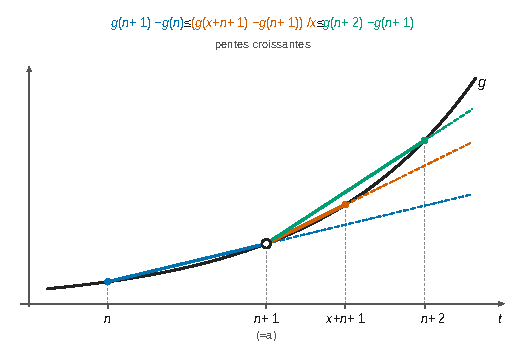
\includegraphics{figures/q17-cordes-lemme-des-pentes.pdf}
\caption*{Figure 1 --- Les trois cordes issues de (n + 1, g(n + 1)) : leurs pentes
croissent avec l'autre extrémité, d'où l'encadrement de Q17 (allure
d'une fonction convexe quelconque)}
\end{figure}

\textbf{Q18.} Soient \(x\in\,]0,1]\) et \(n\in\mathbb N^*\). Par Q15, \(g(n)=\ln((n-1)!)\), \(g(n+1)=\ln(n!)\) et \(g(n+2)=\ln((n+1)!)\). Donc :

\equationajustee{g(n+1)-g(n)=\ln n}

\equationajustee{g(n+2)-g(n+1)=\ln(n+1)}

Par Q16, \(g(x+n+1)-g(n+1)=g(x)+\ln\big(x(x+1)\cdots(x+n)\big)-\ln(n!)\). En multipliant l'encadrement de Q17 par \(x>0\) :

\equationajustee{x\ln n\le g(x)+\ln\frac{x(x+1)\cdots(x+n)}{n!}\le x\ln(n+1).}

Posons \(u_n(x)=\dfrac{n^x\,n!}{x(x+1)\cdots(x+n)}\), de sorte que \(\ln u_n(x)=x\ln n-\ln\frac{x(x+1)\cdots(x+n)}{n!}\). L'encadrement s'écrit :

\equationajustee{\begin{aligned}
0&\le g(x)-\ln u_n(x)\\
&\le x\ln\Big(1+\frac1n\Big)\\
&\le\ln\Big(1+\frac1n\Big).
\end{aligned}}

Le majorant tend vers \(0\) quand \(n\to+\infty\). Par encadrement, \(\ln u_n(x)\to g(x)\). Par continuité de \(\exp\), \(u_n(x)\to e^{g(x)}=f(x)\) :

\equationajustee{\boxed{\forall x\in\,]0,1],\ \ f(x)=\lim_{n\to+\infty}\frac{n^x\,n!}{x(x+1)\cdots(x+n)}.}}

\textbf{Q19.} D'après Q14, \(\Gamma\) est une fonction de \(\mathbb R_+^*\) dans \(\mathbb R_+^*\) qui vérifie \((S)\). Les questions Q15 à Q18 n'utilisent que ces hypothèses : elles s'appliquent à \(\Gamma\).

Pour \(x\in\,]0,1]\), \(\Gamma(x)\) est donc la limite de la même suite \((u_n(x))\), qui ne dépend que de \(x\). Par unicité de la limite :

\equationajustee{\boxed{\forall x\in\,]0,1],\ \ f(x)=\Gamma(x).}}

\textbf{Q20.} Soit \(x>0\). Les intervalles \(]n,n+1]\), \(n\in\mathbb N\), recouvrent \(\mathbb R_+^*\) : il existe \(n\in\mathbb N\) tel que \(y=x-n\in\,]0,1]\).

Par Q15 appliquée à \(f\) et à \(\Gamma\) (qui vérifie \((S)\)), puis Q19 :

\equationajustee{\begin{aligned}
f(x)&=y(y+1)\cdots(y+n-1)\,f(y)\\
&=y(y+1)\cdots(y+n-1)\,\Gamma(y)\\
&=\Gamma(x).
\end{aligned}}

\equationajustee{\boxed{f=\Gamma\ :\ \Gamma\text{ est l'unique fonction }\mathbb R_+^*\to\mathbb R_+^*\text{ \text{vérifiant} }(S).}}

\begin{center}\rule{0.5\linewidth}{0.5pt}\end{center}

Problème --- Étude d'une classe d'endomorphismes

\hypertarget{partie-i---deux-exemples}{%
\section{Partie I - Deux exemples}\label{partie-i---deux-exemples}}

\(E=\mathbb K_2[X]\), de base canonique \(\mathcal B_0=(1,X,X^2)\).

\hypertarget{uxe9tude-de-u}{%
\subsection{\texorpdfstring{Étude de \(u\)}{Étude de u}}\label{uxe9tude-de-u}}

\textbf{Q21.} On a \(u(1)=0\), \(u(X)=1\) et \(u(X^2)=2X^2+2X\). On range en colonnes les coordonnées des images :

\equationajustee{\boxed{A={\mathrm{Mat}}_{\mathcal B_0}(u)=\begin{pmatrix}0&1&0\\0&0&2\\0&0&2\end{pmatrix}.}}

\(A\) est triangulaire supérieure, donc \(\chi_u=X^2(X-2)\) : les valeurs propres sont \(0\) (double) et \(2\) (simple), et \(\chi_u\) est scindé.

Pour \(P=a+bX+cX^2\), on a \(u(P)=b+2cX+2cX^2\). Donc \(\ker u=\mathrm{Vect}(1)\) est de dimension \(1\), strictement inférieure à la multiplicité \(2\) de la valeur propre \(0\).

\equationajustee{\boxed{u\text{ n'est pas diagonalisable.}}}

\textbf{Q22.} Pour \(P=a+bX+cX^2\) :

\equationajustee{u^2(P)=u(b+2cX+2cX^2)=2c+4cX+4cX^2.}

Donc \(u^2(P)=0\) si et seulement si \(c=0\) :

\equationajustee{\boxed{\ker u^2=\mathbb K_1[X]=\mathrm{Vect}(1,X).}}

C'est un sous-espace vectoriel, comme noyau d'un endomorphisme. Il est stable par \(u\), car \(u\) et \(u^2\) commutent : si \(u^2(P)=0\), alors \(u^2(u(P))=u(u^2(P))=0\).

\textbf{Q23.} On cherche une base \((P_1,P_2,P_3)\) telle que \(u(P_1)=2P_1\), \(u(P_2)=0\) et \(u(P_3)=P_2\).

Pour \(P_1=a+bX+cX^2\), l'équation \(u(P_1)=2P_1\) s'écrit \(b=2a\), \(2c=2b\) et \(2c=2c\). On prend \(a=1\) :

\equationajustee{P_1=1+2X+2X^2}

On prend ensuite \(P_2=1\) et \(P_3=X\), qui vérifient \(u(1)=0\) et \(u(X)=1\).

La matrice des coordonnées de \((P_1,P_2,P_3)\) dans \(\mathcal B_0\) est \(\begin{pmatrix}1&1&0\\2&0&1\\2&0&0\end{pmatrix}\), de déterminant \(2\neq0\). Donc \(\mathcal B=(1+2X+2X^2,\,1,\,X)\) est une base de \(E\) et :

\equationajustee{\boxed{{\mathrm{Mat}}_{\mathcal B}(u)=\begin{pmatrix}2&0&0\\0&0&1\\0&0&0\end{pmatrix}.}}

Cette matrice est diagonale par blocs : un bloc \((2)\) de taille \(1\) et un bloc \(\begin{pmatrix}0&1\\0&0\end{pmatrix}\) de taille \(2\). Avec \(p=q=1\), on a \(p+2q=3\) et l'assertion (ii) est vérifiée :

\equationajustee{\boxed{u\in\mathcal D.}}

Autrement dit, \(E=\mathrm{Vect}(P_1)\oplus\mathbb K_1[X]\), somme d'une droite et d'un plan stables.

\hypertarget{uxe9tude-de-v}{%
\subsection{\texorpdfstring{Étude de \(v\)}{Étude de v}}\label{uxe9tude-de-v}}

\textbf{Q24.} On a \(v(1)=0\), \(v(X)=1\) et \(v(X^2)=2X\) :

\equationajustee{\boxed{{\mathrm{Mat}}_{\mathcal B_0}(v)=\begin{pmatrix}0&1&0\\0&0&2\\0&0&0\end{pmatrix}.}}

Cette matrice est triangulaire à diagonale nulle : \(\chi_v=X^3\), et \(0\) est la seule valeur propre de \(v\), avec \(\ker v=\mathrm{Vect}(1)\).

\textbf{Q25.} Soit \(D=\mathrm{Vect}(P)\) une droite, avec \(P\neq0\).

Si \(D\) est stable par \(v\), alors \(v(P)\in D\) : il existe \(\lambda\in\mathbb K\) tel que \(P'=\lambda P\), et \(P\) est un vecteur propre.

Réciproquement, si \(P'=\lambda P\), la droite \(D\) est stable. Les droites stables sont donc exactement les droites engendrées par un vecteur propre de \(v\).

Par Q24, la seule valeur propre est \(0\), et le sous-espace propre associé est \(\ker v=\mathrm{Vect}(1)\).

On peut aussi le voir directement. Supposons \(\lambda\neq0\) et \(P'=\lambda P\), et comparons les degrés.

Si \(\deg P\ge1\), alors \(\deg P'<\deg(\lambda P)\) ; si \(P\) est constant, alors \(P'=0\). Dans les deux cas \(P=0\), ce qui est exclu.

\equationajustee{\boxed{\text{La seule droite stable par }v\text{ est }\mathbb K_0[X]=\mathrm{Vect}(1).}}

\textbf{Q26.} \(\mathbb K_1[X]\) est de dimension \(2\) et stable, car \(v(a+bX)=b\in\mathbb K_1[X]\).

Unicité. Soit \(F\) un plan stable par \(v\), et supposons que \(F\) contienne un polynôme \(P\) de degré \(2\).

Par stabilité, \(F\) contient aussi \(v(P)=P'\), de degré \(1\), et \(v^2(P)=P''\), constante non nulle.

Ces trois polynômes ont des degrés distincts \(2\), \(1\), \(0\) : ils forment une famille libre. Alors \(\dim F\ge3\), ce qui contredit \(\dim F=2\).

Donc \(F\subset\mathbb K_1[X]\), et l'égalité des dimensions donne \(F=\mathbb K_1[X]\).

\equationajustee{\boxed{\mathbb K_1[X]\text{ est le seul plan stable par }v.}}

\textbf{Q27.} Supposons \(v\in\mathcal D\). Par (i), il existe \((p,q)\in\mathbb N^2\) avec \(p+2q=3\), et des sous-espaces stables (droites \(D_i\), plans \(P_j\)) tels que \(E=\bigoplus D_i\oplus\bigoplus P_j\).

Les seules possibilités sont \((p,q)=(3,0)\) et \((p,q)=(1,1)\).

\begin{itemize}
\tightlist
\item
  Cas \((3,0)\) : il faudrait trois droites stables en somme directe, donc distinctes. C'est impossible, car il n'y en a qu'une (Q25).
\item
  Cas \((1,1)\) : par Q25 et Q26, \(D_1=\mathrm{Vect}(1)\) et \(P_1=\mathbb K_1[X]\). Or \(1\in\mathbb K_1[X]\), donc \(D_1\cap P_1\neq\{0\}\) et la somme n'est pas directe.
\end{itemize}

\equationajustee{\boxed{v\notin\mathcal D.}}

\begin{figure}[H]
\centering
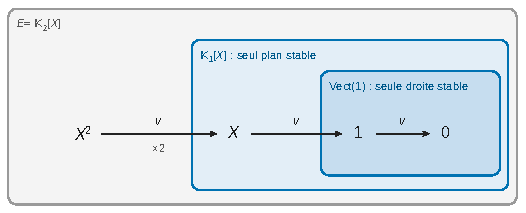
\includegraphics{figures/q25-q27-chaine-de-v.pdf}
\caption*{Figure 2 --- Action de v sur la base canonique : Vect(1) et Vect(1, X),
seuls sous-espaces stables de dimension 1 et 2, sont emboîtés}
\end{figure}

\textbf{Q28.} Soit \(w\in\mathcal L(E)\) défini par \(w(P)=X^2P''\). On a \(w(1)=0\), \(w(X)=0\) et \(w(X^2)=2X^2\).

La matrice de \(w\) dans \(\mathcal B_0\) est \(\mathrm{diag}(0,0,2)\) : elle est diagonale, donc \(w\in\mathcal D\) (trois blocs de taille \(1\)).

Par définition, \(u=w+v\), donc \(v=u-w\). Or \(u\in\mathcal D\) (Q23), \(w\in\mathcal D\), mais \(v\notin\mathcal D\) (Q27). La partie \(\mathcal D\) n'est donc pas stable par combinaison linéaire.

\equationajustee{\boxed{\mathcal D\text{ n'est pas un sous-espace vectoriel de }\mathcal L(E).}}

\hypertarget{partie-ii---le-cas-des-endomorphismes-nilpotents}{%
\section{Partie II - Le cas des endomorphismes nilpotents}\label{partie-ii---le-cas-des-endomorphismes-nilpotents}}

\hypertarget{cas-n1}{%
\subsection{\texorpdfstring{Cas \(n=1\)}{Cas n=1}}\label{cas-n1}}

\textbf{Q29.} Soit \((e)\) une base de \(E\), de dimension \(1\). Comme \(u(e)\in\mathrm{Vect}(e)\), il existe \(\lambda\in\mathbb K\) tel que \(u(e)=\lambda e\).

Par linéarité, \(u=\lambda\,{\mathrm{Id}}_E\).

Alors \(u^k=\lambda^k{\mathrm{Id}}_E=0\) impose \(\lambda^k=0\), donc \(\lambda=0\).

\equationajustee{\boxed{u=0\ (\text{et }k=1).}}

\hypertarget{cas-n2}{%
\subsection{\texorpdfstring{Cas \(n=2\)}{Cas n=2}}\label{cas-n2}}

\textbf{Q30.} Un tel \(x\) existe : par minimalité de l'indice \(k\), on a \(u^{k-1}\neq0\).

Soit \(\sum_{i=0}^{k-1}\lambda_iu^i(x)=0\) et supposons les \(\lambda_i\) non tous nuls. Soit \(i_0\) le plus petit indice tel que \(\lambda_{i_0}\neq0\).

Appliquons \(u^{k-1-i_0}\). Pour \(i>i_0\), le terme devient \(\lambda_iu^{k-1+(i-i_0)}(x)\), nul car l'exposant est au moins \(k\).

Il reste \(\lambda_{i_0}u^{k-1}(x)=0\). Comme \(u^{k-1}(x)\neq0\), on obtient \(\lambda_{i_0}=0\) : contradiction.

\equationajustee{\boxed{\big(u^{k-1}(x),\dots,u(x),x\big)\text{ est libre.}}}

\textbf{Q31.} La famille libre de Q30 compte \(k\) vecteurs dans un espace de dimension \(2\) : son cardinal est au plus la dimension, donc \(k\le2\).

Par ailleurs \(k\ne1\) : sinon \(u=u^1=0\), alors que \(u\) est supposé non nul. Comme \(k\in\mathbb N^*\), on a \(k\ge2\).

\equationajustee{\boxed{k=2\ \text{ et }\ u^2=0,\ \text{ donc }\ u\in\mathcal N_2.}}

\hypertarget{cas-guxe9nuxe9ral}{%
\subsection{Cas général}\label{cas-guxe9nuxe9ral}}

\textbf{Q32.} Soit \(u\in\mathcal D\cap\mathcal N\), d'indice \(k\). Soit \(E=\bigoplus_iD_i\oplus\bigoplus_jP_j\) une décomposition donnée par (i).

Pour chaque facteur \(F\), stable par \(u\), l'endomorphisme induit \(u_F\) vérifie \(u_F^k=(u^k)_F=0\) : il est nilpotent.

\begin{itemize}
\tightlist
\item
  Si \(\dim F=1\), Q29 donne \(u_F=0\).
\item
  Si \(\dim F=2\), ou bien \(u_F=0\), ou bien Q31 appliquée à \(u_F\) donne \(u_F^2=0\).
\end{itemize}

Dans tous les cas \(u_F^2=0\). Tout \(x\in E\) s'écrit \(x=\sum_Fx_F\) avec \(x_F\in F\), donc \(u^2(x)=\sum_Fu_F^2(x_F)=0\).

\equationajustee{\boxed{\mathcal D\cap\mathcal N\subset\mathcal N_2.}}

\textbf{Q33.} Soit \(y=u(x)\in\mathrm{Im}\,u\). Alors \(u(y)=u^2(x)=0\), donc \(y\in\ker u\).

Le théorème du rang donne \(\dim\ker u=n-r\). L'inclusion donne alors \(r=\dim\mathrm{Im}\,u\le\dim\ker u\) :

\equationajustee{\boxed{\mathrm{Im}\,u\subset\ker u\ \text{ et }\ r\le n-r.}}

\textbf{Q34.} La construction a un sens. La famille \((e_1,\dots,e_r)\) est libre et contenue dans \(\ker u\) (Q33) : on peut la compléter en une base de \(\ker u\), de dimension \(n-r\).

Les \(f_i\) existent, car chaque \(e_i\) avec \(i\le r\) appartient à \(\mathrm{Im}\,u\).

La famille compte \((n-r)+r=n=\dim E\) vecteurs : il suffit de montrer qu'elle est libre. Soient des scalaires \(\lambda_1,\dots,\lambda_{n-r}\) et \(\mu_1,\dots,\mu_r\) tels que :

\equationajustee{\sum_i\lambda_ie_i+\sum_j\mu_jf_j=0.}

En appliquant \(u\), comme \(e_i\in\ker u\) et \(u(f_j)=e_j\), on obtient \(\sum_j\mu_je_j=0\). La famille \((e_1,\dots,e_r)\) est libre, donc tous les \(\mu_j\) sont nuls.

Il reste \(\sum_i\lambda_ie_i=0\). La liberté de la base \((e_1,\dots,e_{n-r})\) de \(\ker u\) donne \(\lambda_i=0\) pour tout \(i\).

\equationajustee{\boxed{(e_1,\dots,e_{n-r},f_1,\dots,f_r)\text{ est une base de }E.}}

\textbf{Q35.} On réordonne la base de Q34 :

\equationajustee{\mathcal B=(e_{r+1},\dots,e_{n-r},\,e_1,f_1,\,e_2,f_2,\dots,e_r,f_r).}

C'est une base de \(E\), et \(n-2r\ge0\) par Q33.

On a \(u(e_i)=0\) pour tout \(i\), car les \(e_i\) sont dans \(\ker u\), et \(u(f_i)=e_i\) pour \(i\le r\).

Les \(n-2r\) premières colonnes de la matrice sont nulles. Chaque couple \((e_i,f_i)\) engendre un plan stable, sur lequel la matrice de \(u\) dans la base \((e_i,f_i)\) est \(\begin{pmatrix}0&1\\0&0\end{pmatrix}=J\) :

\equationajustee{\boxed{{\mathrm{Mat}}_{\mathcal B}(u)=\mathrm{diag}\big(0_{n-2r},\underbrace{J,\dots,J}_{r}\big).}}

\begin{figure}[H]
\centering
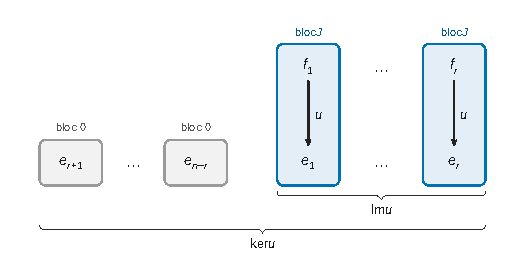
\includegraphics{figures/q33-q35-base-adaptee-n2.pdf}
\caption*{Figure 3 --- Base de Q35 pour u² = 0 : chaque paire (eᵢ, fᵢ) donne un
bloc J, chaque eⱼ avec j \textgreater{} r un bloc nul}
\end{figure}

\textbf{Q36.} L'inclusion \(\mathcal D\cap\mathcal N\subset\mathcal N_2\) est Q32.

Réciproquement, soit \(u\in\mathcal N_2\). Comme \(u^2=0\), \(u\) est nilpotent.

Dans la base de Q35, sa matrice est diagonale par blocs : \(p=n-2r\) blocs nuls de taille \(1\) et \(q=r\) blocs \(J\) de taille \(2\).

Comme \(p+2q=n\), l'assertion (ii) donne \(u\in\mathcal D\).

\equationajustee{\boxed{\mathcal N_2=\mathcal D\cap\mathcal N.}}

\hypertarget{partie-iii---un-crituxe8re-dappartenance-uxe0-mathcal-d}{%
\section{\texorpdfstring{Partie III - Un critère d'appartenance à \(\mathcal D\)}{Partie III - Un critère d'appartenance à \textbackslash mathcal D}}\label{partie-iii---un-crituxe8re-dappartenance-uxe0-mathcal-d}}

\textbf{Q37.} \emph{Linéarité.} Pour \((A,B),(A_1,B_1)\in\mathbb K_1[X]^2\) et \(\lambda\in\mathbb K\), la distributivité du produit des polynômes donne :

\equationajustee{\varphi\big((A,B)+\lambda(A_1,B_1)\big)=\varphi(A,B)+\lambda\,\varphi(A_1,B_1).}

\(\varphi\) est donc linéaire (une seule variable, le couple \((A,B)\)). Elle est à valeurs dans \(\mathbb K_3[X]\), car chaque produit est de degré au plus \(2+1=3\).

\emph{Dimensions.} \(\dim\mathbb K_1[X]^2=2+2=4=\dim\mathbb K_3[X]\). Une application linéaire entre deux espaces de même dimension finie est bijective dès qu'elle est injective : il suffit de montrer que \(\ker\varphi=\{0\}\).

\emph{Injectivité.} Supposons \((X-a)^2A+(X-b)^2B=0\).

\begin{itemize}
\tightlist
\item
  L'évaluation en \(a\) donne \((a-b)^2B(a)=0\), donc \(B(a)=0\) car \(a\neq b\).
\item
  On dérive l'égalité, puis on évalue en \(a\) : \(2(a-b)B(a)+(a-b)^2B'(a)=0\), donc \(B'(a)=0\).
\end{itemize}

Comme \(\deg B\le1\), on a \(B=B(a)+B'(a)(X-a)=0\). Il reste \((X-a)^2A=0\), donc \(A=0\) par intégrité de \(\mathbb K[X]\).

\equationajustee{\boxed{\varphi\text{ est un isomorphisme de }\mathbb K_1[X]^2\text{ sur }\mathbb K_3[X].}}

Par surjectivité, le polynôme \(1\in\mathbb K_3[X]\) a un antécédent :

\equationajustee{\boxed{\exists (A,B)\in\mathbb K_1[X]^2,\ \ (X-a)^2A+(X-b)^2B=1.}}

Par exemple, pour \(a=0\) et \(b=1\) : \(A=3-2X\) et \(B=1+2X\).

\textbf{Q38.} L'application \(P\mapsto P(u)\) est linéaire et vérifie \((PQ)(u)=P(u)\circ Q(u)\) ; en particulier, deux polynômes en \(u\) commutent. En évaluant en \(u\) la relation de Q37 :

\equationajustee{{\mathrm{Id}}_E=A(u)\circ(u-a\,{\mathrm{Id}}_E)^2+B(u)\circ(u-b\,{\mathrm{Id}}_E)^2.}

Soit \(x\) dans les deux noyaux. En appliquant cette égalité à \(x\), on obtient \(x=A(u)(0)+B(u)(0)=0\).

\equationajustee{\boxed{\ker(u-a\,{\mathrm{Id}}_E)^2\cap\ker(u-b\,{\mathrm{Id}}_E)^2=\{0\}.}}

\textbf{Q39.} Récurrence sur \(p\). Pour \(p\le1\), il n'y a rien à montrer. Supposons le résultat vrai pour \(p-1\) scalaires distincts.

Soient \(x_i\in\ker(u-\alpha_i\,{\mathrm{Id}}_E)\), pour \(1\le i\le p\), avec \(\sum_{i=1}^px_i=0\). En appliquant \(u-\alpha_p{\mathrm{Id}}_E\), on obtient :

\equationajustee{\sum_{i=1}^{p-1}(\alpha_i-\alpha_p)\,x_i=0.}

Chaque terme \((\alpha_i-\alpha_p)x_i\) appartient à \(\ker(u-\alpha_i{\mathrm{Id}}_E)\). Par hypothèse de récurrence, ces termes sont nuls. Comme \(\alpha_i\neq\alpha_p\), on obtient \(x_i=0\) pour \(i<p\), puis \(x_p=0\).

\equationajustee{\boxed{\text{La somme }\textstyle\sum_{i=1}^p\ker(u-\alpha_i{\mathrm{Id}}_E)\text{ est directe.}}}

Certains de ces noyaux peuvent être réduits à \(\{0\}\), ce qui ne change rien.

\textbf{Q40.} Pour \(q\in\mathbb N\), on note \(\mathcal H_q\) la propriété : « pour tout \(p\in\mathbb N\) et tous scalaires \(\alpha_1,\dots,\alpha_p,\beta_1,\dots,\beta_q\) deux à deux distincts, la somme \(\sum_i\ker(u-\alpha_i{\mathrm{Id}}_E)+\sum_j\ker(u-\beta_j{\mathrm{Id}}_E)^2\) est directe ».

\(\mathcal H_0\) est Q39. Supposons \(\mathcal H_q\) vraie. Soient \(\alpha_1,\dots,\alpha_p,\beta_1,\dots,\beta_{q+1}\) deux à deux distincts. Soient \(x_i\in\ker(u-\alpha_i{\mathrm{Id}}_E)\) et \(y_j\in\ker(u-\beta_j{\mathrm{Id}}_E)^2\) tels que :

\equationajustee{\sum_ix_i+\sum_{j=1}^{q+1}y_j=0.}

Appliquons \(w=(u-\beta_{q+1}{\mathrm{Id}}_E)^2\), qui est un polynôme en \(u\) :

\begin{itemize}
\tightlist
\item
  \(w(y_{q+1})=0\) ;
\item
  \(w(x_i)=(\alpha_i-\beta_{q+1})^2x_i\), qui appartient à \(\ker(u-\alpha_i{\mathrm{Id}}_E)\) ;
\item
  pour \(j\le q\), \(w(y_j)\in\ker(u-\beta_j{\mathrm{Id}}_E)^2\), car \(w\) commute avec \((u-\beta_j{\mathrm{Id}}_E)^2\).
\end{itemize}

On obtient :

\equationajustee{\sum_i(\alpha_i-\beta_{q+1})^2x_i+\sum_{j\le q}w(y_j)=0.}

Par \(\mathcal H_q\), chaque terme est nul. Comme \(\alpha_i\neq\beta_{q+1}\), on a \(x_i=0\).

Pour \(j\le q\), \(w(y_j)=0\) : le vecteur \(y_j\) appartient à \(\ker(u-\beta_{q+1}{\mathrm{Id}}_E)^2\cap\ker(u-\beta_j{\mathrm{Id}}_E)^2\), réduit à \(\{0\}\) par Q38.

Il reste \(y_{q+1}=0\) : \(\mathcal H_{q+1}\) est vraie.

\equationajustee{\boxed{\text{La somme }\bigoplus_{i=1}^p\ker(u-\alpha_i{\mathrm{Id}}_E)\oplus\bigoplus_{j=1}^q\ker(u-\beta_j{\mathrm{Id}}_E)^2\text{ est directe.}}}

\textbf{Q41.} Soit \(N=p+2q=\deg P\ge1\).

Les \(P_i\) et les \(Q_j\) sont de degré \(N-1\), les \(R_j\) de degré \(N-2\) : tous sont dans \(\mathbb K_{N-1}[X]\).

La famille compte \(p+2q=N=\dim\mathbb K_{N-1}[X]\) éléments. Soit une combinaison linéaire nulle :

\equationajustee{\sum_i\lambda_iP_i+\sum_j\big(\mu_jQ_j+\nu_jR_j\big)=0.}

\begin{itemize}
\tightlist
\item
  Évaluation en \(\alpha_{i_0}\). Tous les polynômes de la famille sauf \(P_{i_0}\) contiennent le facteur \(X-\alpha_{i_0}\). Et \(P_{i_0}(\alpha_{i_0})\neq0\) :
\end{itemize}

\equationajustee{P_{i_0}(\alpha_{i_0})=\prod_{l\neq i_0}(\alpha_{i_0}-\alpha_l)\prod_j(\alpha_{i_0}-\beta_j)^2.}

Donc \(\lambda_{i_0}=0\).

\begin{itemize}
\item
  Évaluation en \(\beta_{j_0}\). Les \(P_i\), ainsi que \(Q_j\) et \(R_j\) pour \(j\neq j_0\), contiennent le facteur \((X-\beta_{j_0})^2\).

  De plus \(Q_{j_0}=(X-\beta_{j_0})R_{j_0}\) s'annule en \(\beta_{j_0}\). Enfin \(R_{j_0}(\beta_{j_0})\neq0\) :
\end{itemize}

\equationajustee{R_{j_0}(\beta_{j_0})=\prod_i(\beta_{j_0}-\alpha_i)\prod_{l\neq j_0}(\beta_{j_0}-\beta_l)^2.}

Donc \(\nu_{j_0}=0\).

\begin{itemize}
\item
  Il reste \(\sum_j\mu_jQ_j=0\). On dérive, puis on évalue en \(\beta_{j_0}\).

  Pour \(j\neq j_0\), \((X-\beta_{j_0})^2\) divise \(Q_j\), donc \(Q_j'(\beta_{j_0})=0\). Et \(Q_{j_0}'(\beta_{j_0})=R_{j_0}(\beta_{j_0})\neq0\). Donc \(\mu_{j_0}=0\).
\end{itemize}

La famille est libre, de cardinal \(\dim\mathbb K_{N-1}[X]\) :

\equationajustee{\boxed{\mathcal B=(P_1,\dots,P_p,Q_1,\dots,Q_q,R_1,\dots,R_q)\text{ est une base de }\mathbb K_{p+2q-1}[X].}}

\textbf{Q42.} Comme \(N\ge1\), le polynôme \(1\) appartient à \(\mathbb K_{N-1}[X]\). Il existe donc des scalaires tels que :

\equationajustee{1=\sum_i\lambda_iP_i+\sum_j\big(\mu_jQ_j+\nu_jR_j\big).}

On évalue en \(u\) et on applique à \(x\in E\) :

\equationajustee{x=\sum_i\underbrace{\lambda_iP_i(u)(x)}_{x_i}+\sum_j\underbrace{\big(\mu_jQ_j(u)+\nu_jR_j(u)\big)(x)}_{y_j}.}

On utilise \(P(u)=0\) et les relations \((X-\alpha_i)P_i=P\), \((X-\beta_j)^2Q_j=(X-\beta_j)P\) et \((X-\beta_j)^2R_j=P\) :

\equationajustee{(u-\alpha_i{\mathrm{Id}}_E)(x_i)=\lambda_i\,P(u)(x)=0}

\equationajustee{\begin{aligned}
(u-\beta_j{\mathrm{Id}}_E)^2(y_j)&=\mu_j\,(u-\beta_j{\mathrm{Id}}_E)\big(P(u)(x)\big)+\nu_j\,P(u)(x)\\
&=0.
\end{aligned}}

Ainsi \(x_i\in\ker(u-\alpha_i{\mathrm{Id}}_E)\) et \(y_j\in\ker(u-\beta_j{\mathrm{Id}}_E)^2\) : \(E\) est la somme de ces noyaux. Cette somme est directe par Q40 :

\equationajustee{\boxed{\begin{aligned}
E&=\bigoplus_{i=1}^p\ker(u-\alpha_i{\mathrm{Id}}_E)\\
&\qquad\oplus\bigoplus_{j=1}^q\ker(u-\beta_j{\mathrm{Id}}_E)^2.
\end{aligned}}}

\textbf{Q43.} Posons \(E_i=\ker(u-\alpha_i{\mathrm{Id}}_E)\) et \(F_j=\ker(u-\beta_j{\mathrm{Id}}_E)^2\). Ce sont des noyaux de polynômes en \(u\), donc des sous-espaces stables par \(u\). Par Q42, \(E=\bigoplus_iE_i\oplus\bigoplus_jF_j\).

\begin{itemize}
\item
  Sur \(E_i\neq\{0\}\), \(u\) induit \(\alpha_i\mathrm{Id}\) : toute base de \(E_i\) le découpe en droites stables par \(u\).
\item
  Sur \(F_j\neq\{0\}\), l'endomorphisme \(u-\beta_j{\mathrm{Id}}_E\) induit un endomorphisme \(\theta_j\) de \(F_j\), de carré nul.

  On applique Q36 dans l'espace \(F_j\), de dimension au moins \(1\) : \(\theta_j\) appartient à la classe \(\mathcal D\) de \(F_j\).

  Donc \(F_j\) est somme directe de droites et de plans stables par \(\theta_j\).
\item
  Un sous-espace \(G\subset F_j\) stable par \(\theta_j\) est stable par \(u\) : pour \(x\in G\), \(u(x)=\theta_j(x)+\beta_jx\in G\).
\end{itemize}

En réunissant ces décompositions, \(E\) est somme directe de \(p'\) droites et \(q'\) plans stables par \(u\), avec \(p'+2q'=n\) : l'assertion (i) est vérifiée.

Dans une base adaptée, la matrice de \(u\) est diagonale par blocs. Ses blocs sont des \((\alpha_i)\), des \((\beta_j)\) et des \(\begin{pmatrix}\beta_j&1\\0&\beta_j\end{pmatrix}\).

\equationajustee{\boxed{u\in\mathcal D.}}

Ainsi, tout endomorphisme qui admet un polynôme annulateur scindé à racines simples ou doubles appartient à \(\mathcal D\). On peut en effet supposer ce polynôme unitaire, donc de la forme (2), avec \((p,q)\neq(0,0)\) puisque \(E\neq\{0\}\).

FIN

\end{document}
